\subsection{Encryptors}

Note: Write about the Encryption.Core lib (basic constructs, why are there so many similar classes that are held
as different objects? because this is good object oriented design. passing around non-descript byte[] is BAD design).

\begin{figure}[htb]
	\centering
	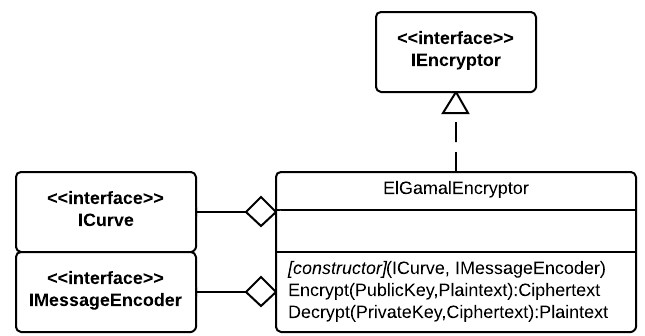
\includegraphics[width=0.7\textwidth]{implementation/encryptors}
	\caption{The only encryptors currently supported rely on public-key cryptography. Like encoders, the encryptors have their state set
		in their constructors, and provide a simple interface for the encryption (\((PublicKey,Plaintext) \to Ciphertext\)) and decryption
		(\((PrivateKey,Ciphertext) \to Plaintext\)) operations themselves. In addition, the encryptors must provide a way to generate a
		random key-pair.}
\end{figure}

Note: The encryption is structured in such a way that it is trivial to add different encryptors to the project. Good
if you want to support hybrid encryptions such as ECIES in the future. ECIES would not require an encoder, either...!
How would the interface need to change to support ECIES? Nothing. It is public-key encryption.
However, symmetric key encryption (is this possible with ECC?) would require a new interface.